\documentclass[a4paper,man,natbib,floatsintext]{apa6}

\usepackage[english]{babel}
\usepackage[utf8x]{inputenc}
\usepackage{amsmath}
\usepackage{graphicx}
\usepackage[colorinlistoftodos]{todonotes}
\usepackage{xcolor}
\usepackage[draft,inline,nomargin,index]{fixme}
\usepackage{hyperref}

\fxsetup{theme=color,mode=multiuser}
\FXRegisterAuthor{ab}{sab}{\color{blue}Amelie} % abnote{} with text inside to edit
\FXRegisterAuthor{bb}{sbb}{\color{purple}Brice} % bbnote{} with text inside to edit
\FXRegisterAuthor{ln}{sln}{\color{violet}Lad} % lnnote{} with text inside to edit

\title{Possible biasedness of the sequential testing procedure}
%\title{Preventing a possible bias of the sequential testing procedure}
%\title{Blinding as a remedy for demand biases during sequential testing}
\shorttitle{Blind Bayes Factor}
\threeauthors{Amélie G. Bret}{Brice Beffara}{Ladislas Nalborczyk}
\threeaffiliations{Univ. Grenoble Alpes, CNRS, LPNC UMR 5105, F-38000, Grenoble \\Psychological Science Research Institute, Catholic University of Louvain, Belgium}{The Walden III Slowpen Science Laboratory, France}{Univ. Grenoble Alpes, CNRS, LPNC UMR 5105, F-38000, Grenoble \\ Department of Experimental Clinical and Health Psychology, Ghent University}

\abstract{When collecting data, Bayesian hypothesis testing allows optional stopping with unlimited multiple testing. This procedure is called Sequential Bayes Factor (SBF). Bayes factors are computed until an a priori defined level of evidence is reached. This allows flexible sampling plans and is not dependent upon correct effect size guesses in an a priori power analysis. Testing mean differences between 2 groups, the SBF design typically needs 50\% to 70\% smaller samples to reach a conclusion about the presence of an effect, as compared with optimal NHST, while having the same or lower long-term rate of wrong inference...however... \todo[inline, color=red]{Le début de l'asbtract est extrait de pain joli et al. Il faudra le reformuler.}}

\begin{document}
\maketitle

\section{Aspects pratiques}

Original papers: \cite{schonbrodt_bayes_2017}, \& \cite{schonbrodt_sequential_2017}...

\lnnote{IMO, un commentaire doit être court (i.e., < 2000-3000 mots), mais il faudrait peut-être qu'on trouve des guidelines précises ?}

\lnnote{Où publier ? S'il s'agit d'un commentaire, il doit être publié dans la même revue que l'article original. Les deux papiers ci-dessus présentent la méthode SBF (à bien relire en détails), un dans Psych. Meth (2017) et l'autre dans PBR (in press). \newline PBR accepte les commentaires (cf. la page d'accueil du journal), mais je ne sais pas si Psychological Methods les accepte...}

\bbnote{Exact mais Psych Meth accepte aussi des tuto donc on pourrait peut-être faire passer ça comme un tuto non ?}

\lnnote{Ça me semble un peu léger pour un tuto... non ? On présenterait quoi ? Juste une fonction qui ajoute un argument "blind" aux fonctions existantes ? Ça ferait un bon article de blog mais je pense que c'est un peu léger pour un tuto...PS: je pense que Psych. Meth. accepte les comments, même s'ils ne le précisent, mais il faudrait juste s'en assurer... je peux m'occuper de vérifier ça}

\section{Proposition de plan}

\renewcommand{\labelenumii}{\Roman{enumii}}
\begin{enumerate}
	\item{Introduction, état du problème}
	\begin{enumerate}
		\item{Présentation de la méthode SBF}
		\item{Problèmes}
			\begin{enumerate}
            \item{Non-respect de l'hypothèse d'indépendance des observations}
            \item{Biais de demande...}
            \end{enumerate}
            \end{enumerate}
            \item{Solutions, comment régler le problème ?}
            \begin{enumerate}
            \item{Blinding: soit triple blind (expé != analyst), soit blinding via software, cf. point suivant}
            \item{On peut proposer ici une solution pratique immédiate, genre une version modifiée de la fonction de félix qui ajouter un argument "blind" (voir supplementary materials)}
            \end{enumerate}
            \item{Evaluation du biais ?}
            \begin{enumerate}
            \item{Propositions de protocoles expérimentaux permettant de mettre en évidence le biais, et prédictions (cf Figure 2).}
            \item{On pourrait profiter de ce papier pour lancer un appel à contribution à une grosse manip multi-lab all around the world, pour évaluer l'amplitude de ce biais, comme on avait commencé à discuter...non ?}

\end{enumerate}
\end{enumerate}

\bbnote{super idée j'aime cet séquence évolutive vmvc}

\section{Sondage et liste des arguments pour ou contre inclure Wagenmakers, Schönbrodt, Perugini et cie ?}

\textbf{Pour}: ils sont forts, ils peuvent nous éviter de dire des bêtises, ça fait moins "attaque" s'ils sont aussi auteurs...

\textbf{Contre}: on peut les avoir en reviewers... et ça fait une diversité de point de vues dans la littérature (genre moins crew)

\section{TO-DO}

\begin{itemize}

\item{trouver un acronyme sexy pour décrire le biais, genre le "Sequential Experimenter-as-Analyst Bias" (SEAB).} \lnnote{DONE ?}

\item{revue de littérature sur le biais de l'expérimentateur, travaux récents ? estimation de la taille d'effet ?}

\item{insérer un diagramme qui représente le processus de sequential testing et là où opère notre biais potentiel...cf section "diagrammes"}\lnnote{DONE, cf. below}

\item{insérer un diagramme de nos prédictions...cf section "diagrammes"}\lnnote{DONE, cf. below}

\item{modifier la fonction seqBF de Richard Morey et Félix Schonbrodt afin d'ajouter un argument "blind"} \lnnote{DONE, cf. attached R script}

\end{itemize}

\section{Introduction}

...what is a Bayes Factor (BF)...and how it avoids the pitfalls of sequential testing  in the Null Hypothesis Significance Testing (NHST) framework...

\begin{equation}
\underbrace{\dfrac{p(H_{0}|D)}{p(H_{1}|D)}}_{posterior\ odds} = \underbrace{\dfrac{p(D|H_{0})}{p(D|H_{1})}}_{bayes\ factor} \times \underbrace{\dfrac{p(H_{0})}{p(H_{1})}}_{prior\ odds}
\end{equation}

\vspace{5mm}

where $p(D|H)$ is called the \emph{evidence}, or the probability of the data given an hypothesis and is basically the average of the probabilities of the data over all values of $\theta$, weighted by their prior probabilities:

\begin{equation}
p(D|H) = \int_{\theta} p(\theta|H) p(D|\theta,H) d\theta
\end{equation}

\vspace{5mm}

...thus, the BF can be seen as an updating index, indicating the researcher how much prior probabilities should be revised (e.g.,\citep{kruschke_bayesian_2017a})...blah blah...

\section{Diagrammes}

...see Figure \ref{fig:diag1} pour un exemple de ce à quoi je pensais en parlant des diagrammes... à améliorer bien entendu... Amélie ? :)...created with https://www.draw.io/ ...

\begin{figure}[H]
  \caption{Overview of the SBF procedure and illustration of possible biases when the experimenter and the data analyst are the same person.}
  \centering
  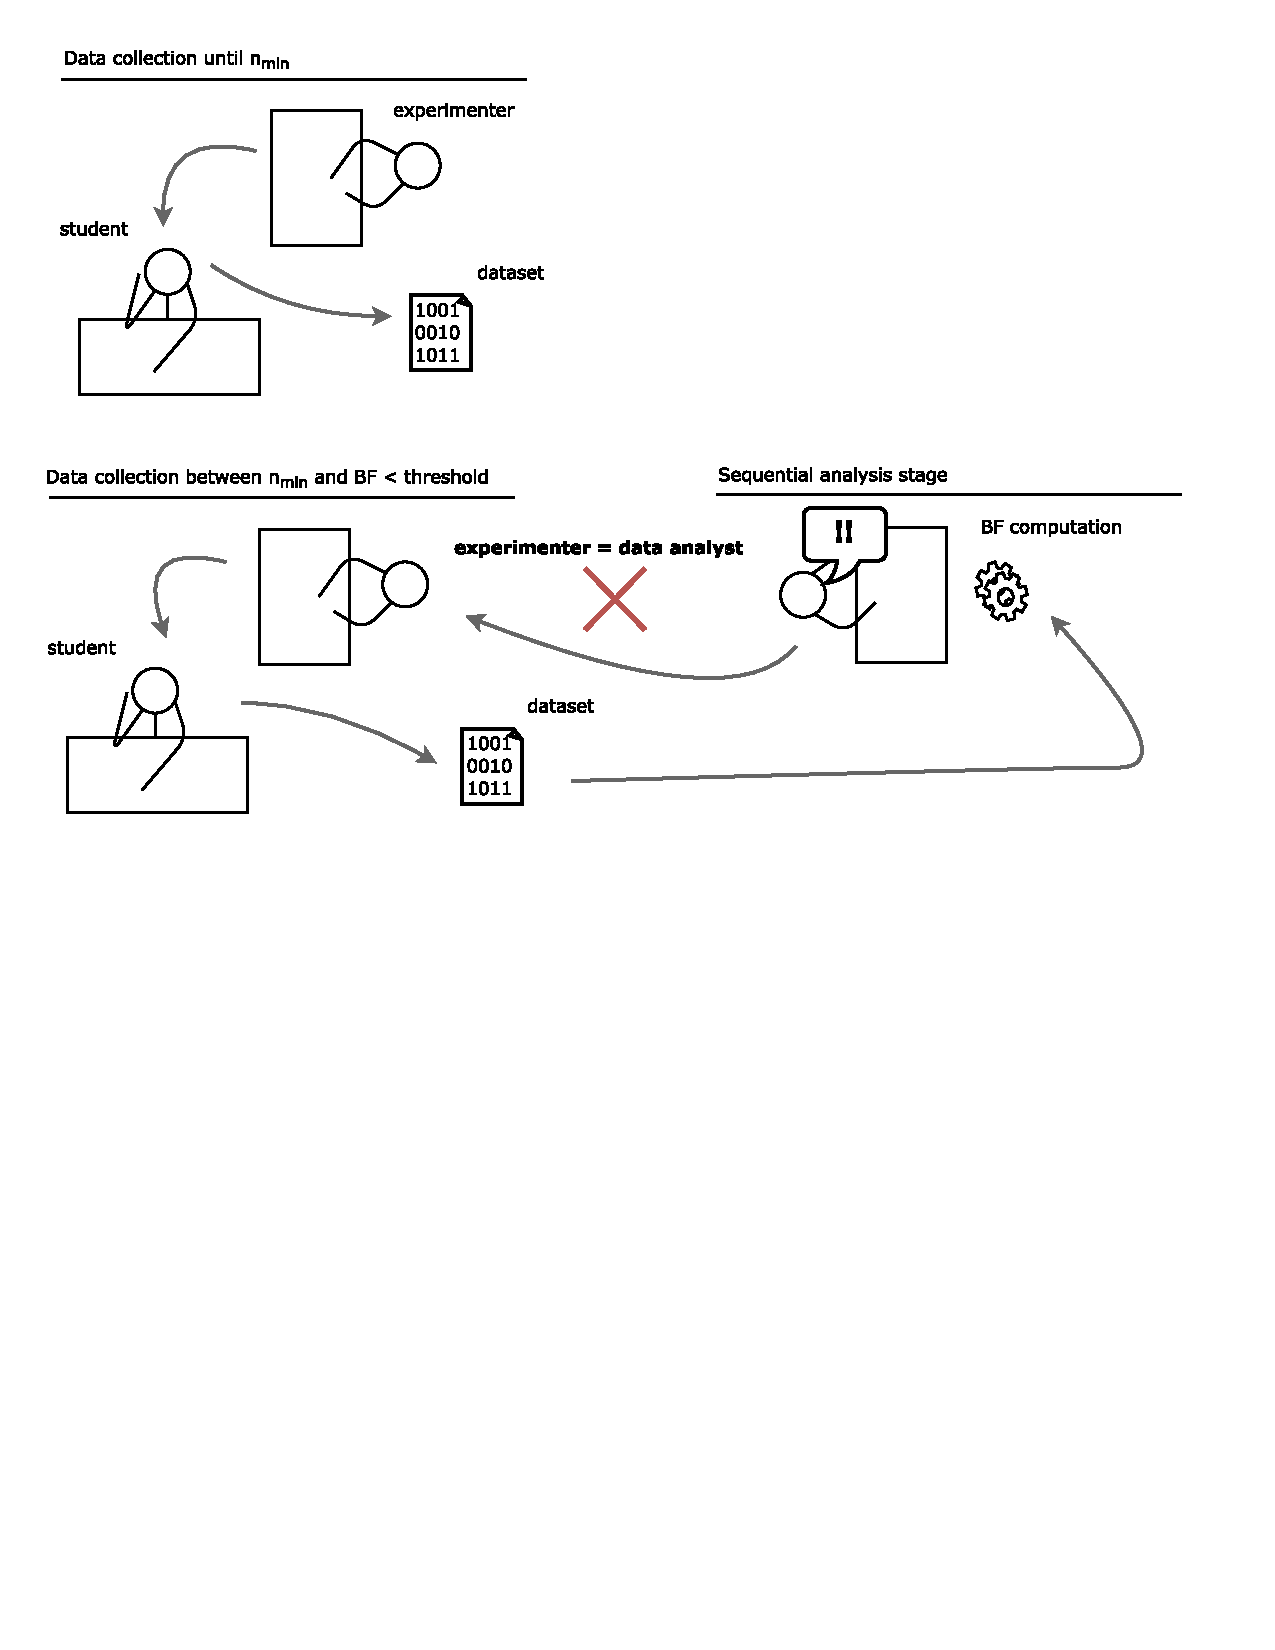
\includegraphics[width=0.8\textwidth]{bias_diag.pdf}
  \label{fig:diag1}
\end{figure}

...la Figure \ref{fig:pred} illustre nos prédictions pour différents scénarios (e.g., l'expé voit une évolution de BF conforme à ses attentes, non-conforme, etc.)...created with https://www.draw.io/ ...

\begin{figure}[H]
  \caption{Predicted consequences of the SEAB on the results of a SBF procedure, for a given Cohen's d of 0.6 (hereafter, "H1") or of 0 (hereafter "H0"), according to the \emph{a priori} researcher's beliefs.}
  \centering
  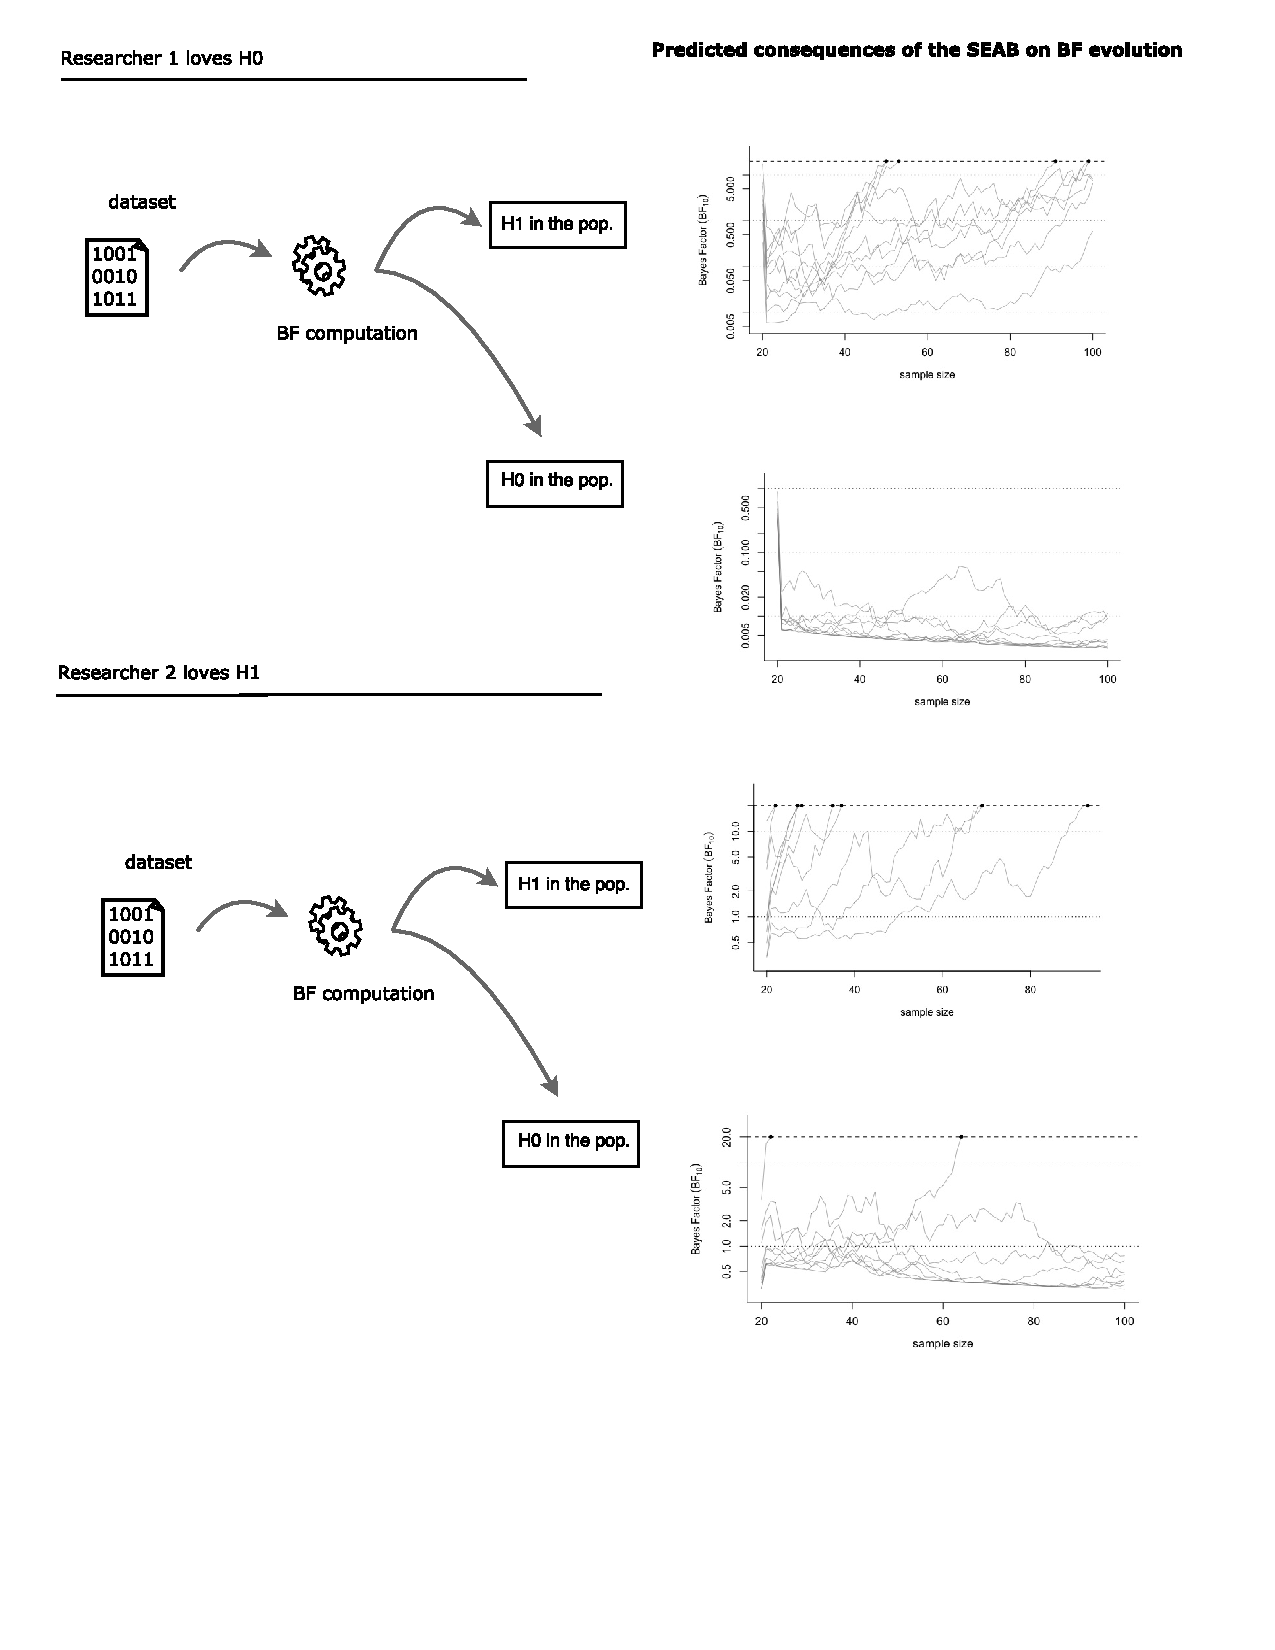
\includegraphics[width=0.8\textwidth]{BFF_predictions.pdf}
  \label{fig:pred}
\end{figure}

...peut-être ajouter un plot de l'évolution "normale" du BF pour cette taille d'effet (i.e., d = 0.6) ?...

...exemple de manip utilisant le SBF: \cite{martin_perceiving_2016}...

\section{Supplementary materials}

...\url{https://github.com/lnalborczyk/Blind_BF}...le repo est privé pour le moment donc on ne peut pas y accéder avec ce lien, mais la fonction est dispo sur le repo Overleaf...

\section{Acknowledgements}

...

% Commands to include a figure:
%\begin{figure}
%\centering
%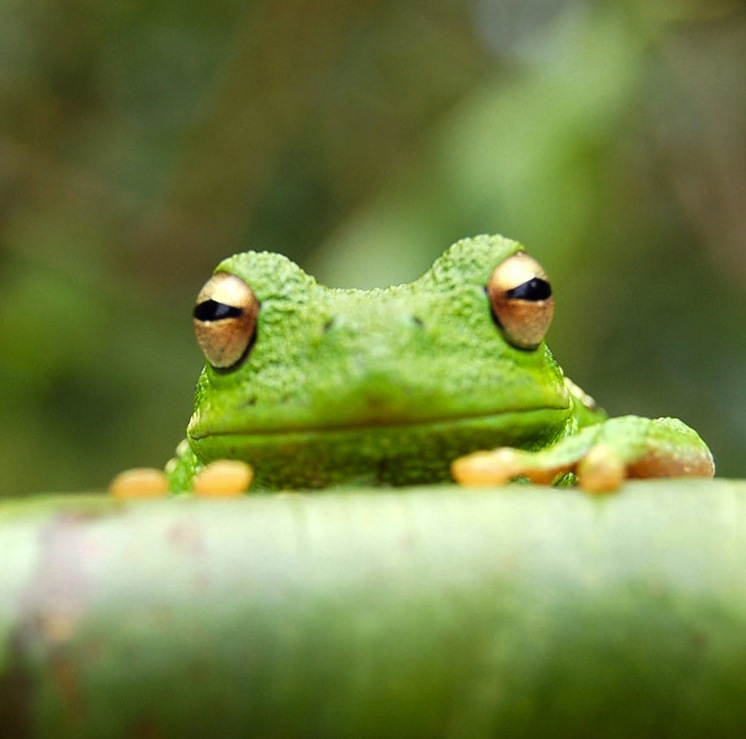
\includegraphics[width=0.5\textwidth]{frog.jpg}
%\caption{\label{fig:frog}This is a figure caption.}
%\end{figure}

\bibliography{BBF}
\end{document}
